%%%%%%%%%%%%%%%%%%%% SECTION %%%%%%%%%%%%%%%%%%%%%%%
\section{Rapid Review research protocol} \label{section:en/protocolo}

This section describes the research protocol used for this rapid review. Rapid Reviews (RR) are practice-oriented secondary studies, and their main goal is to provide evidence to support decision-making towards the solution, or at least attenuation, of issues practitioners face in practice \cite{Cartaxo2020}.

For this Rapid Review, the PRISMA \cite{Tricco2019} methodology was used for reference. The research question for the case study of this work, the repositories used for the search, the search process and search string, the inclusion and exclusion criteria and the selection process are specified as follows.


%%%%%%%%%%%%%%%%%%%% SECTION %%%%%%%%%%%%%%%%%%%%%%%
\subsection{Research Question}

The Research Question to be answered is the following: \emph{What are the main factors that limit the implementation of AI/xAI in histopathology?} Considering all of the impediments reported so far will permit to gather all of the known and necessary requirements to implement AI/xAI in histopathology. 




%%%%%%%%%%%%%%%%%%%% SECTION %%%%%%%%%%%%%%%%%%%%%%%
\subsection{Search Process and Search string} \label{section:en/search_process}

An automatic search in the ACM, IEEE Xplore, PubMed and Springer digital libraries and platforms was conducted.

For the construction of the search string, the main terms “explainable artificial intelligence”, “histopathology”, “histology” and “anatomic pathology” were considered, including their alternative terms. The resulting search string is presented in Figure \ref{figura:en/cadena_generica}.

\begin{figure}[htbp]
\centering
\begin{tabular}{c}
\begin{lstlisting}
#FULL TEXT
  "xai" OR
  "explainable artificial intelligence" OR
  "explainable ai" OR
  "interpretable ai" OR
  "interpretable artificial intelligence" OR
  "white box" OR
  "human ai"
#AND
#FULL TEXT
  "histopathology" OR
  "histopathological" OR
  "histology" OR
  "histological" OR
  "anatomic pathology" OR
  "anatomical pathology"
\end{lstlisting}
\end{tabular}
\caption{Search string defined for the research}
\label{figura:en/cadena_generica}
\end{figure}



%%%%%%%%%%%%%%%%%%%% SECTION %%%%%%%%%%%%%%%%%%%%%%%
\subsection{Inclusion and exclusion criteria} \label{section:en/inc_exc_criteria}


Since 2015, it has been observed an increment of xAI techniques applied to AI clinical decision support systems \cite{Giuste2023}. Based on these dates, the inclusion criteria was defined as follows: articles published in English between January 2015 and June 2023, in journals or conferences that underwent peer review, and whose main focus is the implementation of AI/xAI in histology or histopathology. Duplicate articles, surveys, systematic reviews and other rapid reviews were excluded for this study.



%%%%%%%%%%%%%%%%%%%% SECTION %%%%%%%%%%%%%%%%%%%%%%%
\subsection{Selection and Data Extraction process} \label{section:en/selection_data_process}

The study selection process consisted of ten steps, which were executed sequentially. Details about the process are described in Figure \ref{figura:en/data_extraction}. This process allowed the selection of the primary studies that were analyzed to answer the research question. The PRISMA checklist used in this study is presented in Appendix \ref{appendix:en/prisma_checklist}.

The search string was applied in the digital libraries with some necessary adjustments depending on the particularities of each one.

\begin{figure}[htbp]
    \centering
%    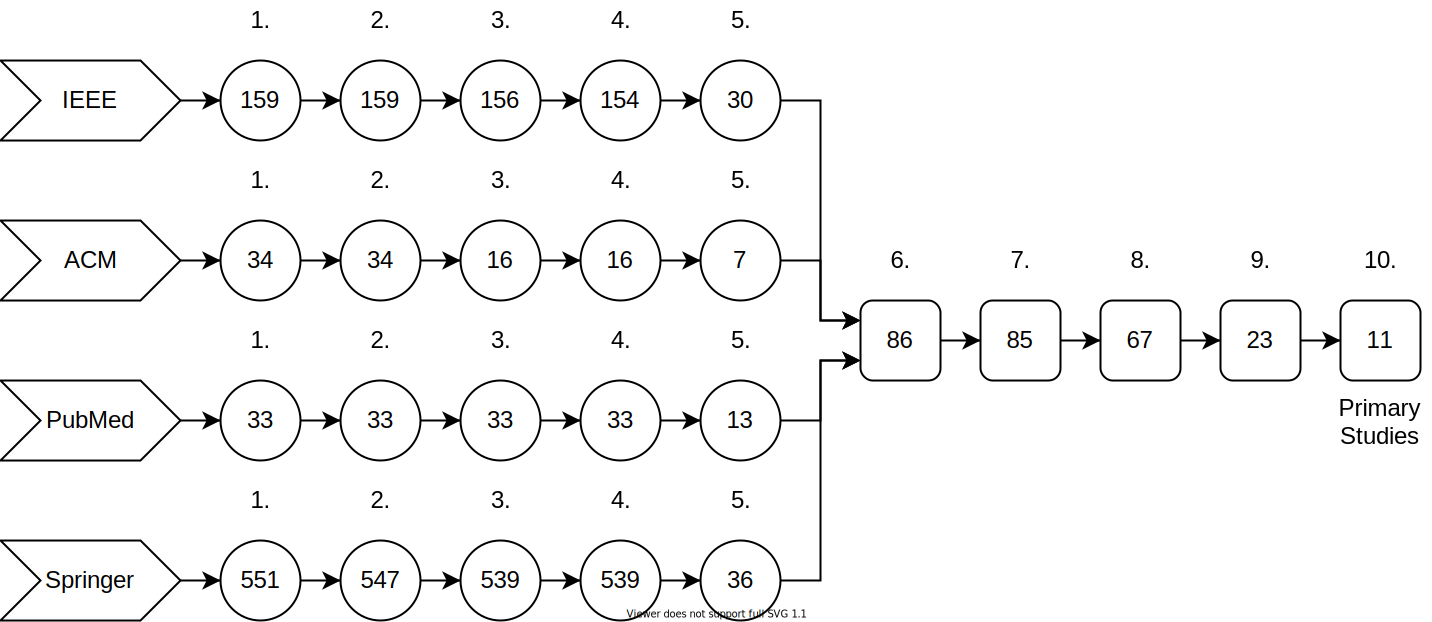
\includegraphics[width=\textwidth]{Imagenes/RR_Steps.svg}
    \includesvg[inkscapelatex=false, width=0.5\textwidth]{Imagenes/RR_Steps_v2.svg}
    \caption{Articles search and selection process details.}
    \label{figura:en/data_extraction}
\end{figure}

For this rapid review, one researcher read the titles, abstracts, and full texts to assess their inclusion. Of a total of 777 articles found, 11 primary studies were analyzed. The list of the selected studies is presented in Appendix \ref{appendix:en/estudios_primarios}.
